\documentclass[tikz]{standalone}

\begin{document}
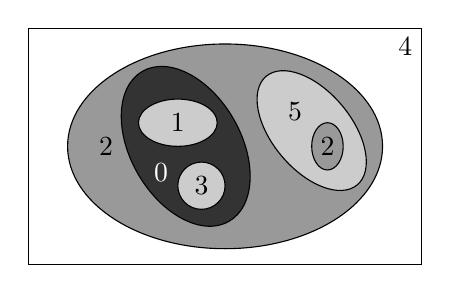
\begin{tikzpicture}
\tikzset{
  shp/.style={},
  shapeO/.prefix style={},
  shapeA/.prefix style={shp,fill=black!40},
  shapeB/.prefix style={shp,fill=black!80},
  shapeC/.prefix style={shp,fill=black!20},
  shapeD/.prefix style={shp,fill=black!20},
  shapeE/.prefix style={shp,fill=black!20},
  shapeF/.prefix style={shp,fill=black!40},
  shplbl/.append style={},
}

\draw (0,0) rectangle (5,3);

\draw[shapeO] (0,0) rectangle (5,3) node[shplbl, below left] {4};

%% Shape A
\draw[shapeA] (2.5,1.5) ellipse (2 and 1.3) node[shplbl,left=1.3cm] {2};

%% Shape B
\draw[shapeB] (2,1.5) circle[x radius=.7, y radius=1.1, rotate=30] node[shplbl, white, below left=.1cm] {0};
%% Shape D
\draw[shapeD] (1.9,1.8) circle[x radius=.5, y radius=.3] node[shplbl] {1};
%% shape E
\draw[shapeE] (2.2,1) circle[x radius=.3, y radius=.3] node[shplbl] {3};
%% Shape C
\draw[shapeC] (3.6,1.7) circle[x radius=.5, y radius=.9, rotate=40] node[shplbl, above left] {5};
%% Shape F
\draw[shapeF] (3.8,1.5) circle[x radius=.2, y radius=.3] node[shplbl] {2};
\end{tikzpicture}
\end{document}